\documentclass[12pt,openright,twoside,a4paper,english,french,spanish]{abntex2}

\input{fixos/pacotes}
\input{fixos/comandos}
\input{fixos/novosComandos}
% Dados pessoais
\autor{Alexandre Torres Kryonidis – 13/0099767 \\Cecília França Dib de Oliveira Bessa – 14/0134425 \\Guilherme Baldissera – 14/0142002 \\	Maria Carolina Machado Ferreira – 14/0153411}
\curso{Engenharia de Software}
% Dados do trabalho
\titulo{Trabalho 2 : Pilates Fit Club}
\data{2016}
\palavraChaveUm{Palavra-chave01}
\palavraChaveDois{Palavra-chave02}
% Dados da orientacao
\orientador{(Titulação Acadêmica e Nome do Orientador)}
\coorientador{(quando houver, Titulação Acadêmica e Nome do Orientador)}
% Dados para a ficha catalográfica
\cdu{02:141:005.6}
% Dados da aprovação do trabalho
\dataDaAprovacao{01 de junho de 2013}
\membroConvidadoUm{Titulação e Nome do Professor Convidado 01}
\membroConvidadoDois{Titulação e Nome do Professor Convidado 02}

\local{Brasília, DF}
\instituicao{%
Universidade de Brasília - UnB
\par
Faculdade UnB Gama - FGA
}
\tipotrabalho{Trabalho de Conclusão de Curso}
\preambulo{Trabalho submetido a disciplina Engenharia de Requisitos do curso de graduação em Engenharia de Software
da Universidade de Brasília.}

\input{fixos/setup}

\begin{document}

\frenchspacing
\imprimircapa
\imprimirfolhaderosto* {}
\pdfbookmark[0]{\listfigurename}{lof}
\listoffigures*
\cleardoublepage
\pdfbookmark[0]{\listtablename}{lot}
\listoftables*
\cleardoublepage

\begin{siglas}
\item[ER] Engenharia de Requisitos
\item[CMMI] Capability Maturity Model - Integration ou Modelo de Maturidade em Capacitação - Integração
\item[MPS.BR] Melhoria do Processo de Software Brasileiro
\item[SAFe] Scaled Agile Framework
\end{siglas}

\input{editaveis/simbolos}
\input{fixos/indiceAutomatico}
\textual
\chapter*[Introdução]{Introdução}
\addcontentsline{toc}{chapter}{Introdução}
Esse projeto tem como objetivo a execução do planejamento feito na primeira
parte do projeto da disciplina Requisitos de Software. Isto é, aplicar no
contexto de desenvolvimento do software, para a empresa  Pilates Fit Club,
atividades relacionadas a Engenharia de Requisitos.

\chapter[Contexto da Organização]{Contexto da Organização}
Aqui deve ser escrito o contexto da organização, escopo global.

\section[Processo de Negócio]{Processo de Negócio}
Aqui deve ser escrito o Processo de Negócio.

\chapter[Abordagem de Engenharia de Requisitos]{Abordagem de Engenharia de Requisitos}
Aqui deve ser escrito a Abordagem de Engenharia de Requisitos, escopo global.

\section[Problema]{Problema}
\begin{quote} Os problemas encontrados são ocasionados pelos fato dos processos não serem automatizados. Segue abaixo exemplos enfrentados pela cliente:
    \begin{itemize}
        \item Todo final de mês a cliente olha todos os contratos para gerar uma lista com os alunos que vencerão no mês subsequente;
		\item Todo final de mês a cliente olha todos os contratos para gerar uma lista com os aniversariantes de próximo mês;
		\item Quando deseja visualizar qualquer dado de um aluno ou informações de seu contrato (telefone, vencimento, dia de pagamento, valor do plano contratado), a cliente procura o contrato deste aluno em específico para visualizar;
		\item A cliente não tem um controle de alunos ativos e inativos;
		\item O controle financeiro (crédito e débito) é parcial e feito manualmente.
    \end{itemize}
\end{quote}
\section[Necessidades]{Necessidades}
\begin{quote}
    \begin{itemize}
        \item Visualizar dados dos alunos e informações dos planos de contrato com mais facilidade;
		\item Obter uma lista com os planos de alunos que irão vencer no mês subsequente;
		\item Obter uma lista com os aniversariantes do mês subsequente;
		\item Obter uma lista com os alunos ativos e inativos;
		\item Visualizar entradas e saídas com mais facilidade.
    \end{itemize}
\end{quote}
\section[Caracteristicas]{Caracteristicas}

\section[UserStories]{UserStories}
\subsection[Visualizar Agenda Diária]{Visualizar Agenda Diária}
Eu como usuário administrador quero visualizar agenda diária para
me certificar de quais alunos tiveram ou terão acesso ao estabelecimento
em determinada data para aula.

\subsection[Visualizar Horário Específico]{VisualizarHorário Específico}
Eu como usuário administrador quero visualizar a agenda referente a um horário
específico para me certificar de quais alunos tiveram ou terão acesso ao
estabelecimento em determinado momento do dia para aula.

\subsection[Visualizar Agenda Semanal]{Visualizar Agenda Semanal}
Eu como usuário administrador quero visualizar a agenda semanal para assim me
certificar de quais alunos tiveram ou terão acesso ao estabelecimento durante tal
semana para aulas.

\subsection[Visualizar Agenda Mensal]{Visualizar Agenda Mensal}
Eu como usuário administrador quero visualizar a agenda mensal para me
certificar de quais alunos tiveram ou terão acesso ao estabelecimento durante
determinado mês para aulas.

\subsection[Gerar Relatório Diário de Aulas]{Gerar Relatório Diário de Aulas}
Eu como usuário administrador quero gerar um relatório diário de aulas para me
certificar de quais alunos compareceram ou não a aula agendada.

\subsection[Criar Aulas]{Criar Aulas}
Essa história de usuário tem como objetivo o desenvolvimento da \textsl{model} referente
a Aulas. Assim permitindo que sejam feitas dependências internas entre aluno
e aulas.

\begin{quote}
Critérios de aceitação:
    \begin{itemize}
        \item O sistema deve permitir registrar novas aulas.
    \end{itemize}
\end{quote}

\subsection[Cadastrar Plano de Contrato]{Cadastrar Plano de Contrato}
Eu como usuário administrador quero cadastrar planos de contratos com as
informações de: quantidade de vezes por semana, período do plano em meses,
valor mensal e percentual de desconto baseado no plano de 1 mês.

\begin{quote}
Critérios de Aceitação:
    \begin{itemize}
        \item O sistema deve permitir a edição de um ou mais dados de planos de contrato
        como o preço da mensalidade e o desconto.
    \end{itemize}
\end{quote}

\subsection[Submeter Contrato]{Submeter Contrato}
Eu como usuário administrador quero realizar o \textsl{upload} de contratos nos formatos
PDF, doc com seu respectivo título e descrição para que eu possua um controle
sobre os antigos contratos e possa imprimir os atuais.

\subsection[Visualizar Contrato]{Visualizar Contrato}
Eu como usuário administrador quero visualizar a lista dos documentos hospedados
(listados pelo seu respectivo título) e abrir esses documentos para que eu possa
visualizar uma lista dos arquivos disponíveis no sistema e realizar o \textsl{download}
de cada um deles.

\subsection[Remover Contrato]{Remover Contrato}
Eu como usuário administrador quero remover do sistema os contratos hospedados
para que eu possa remover os que não são mais importantes e possua controle
sobre os contratos.

\subsection[Cadastrar Professor]{Cadastrar Professor}
Eu como usuário administrador quero cadastrar os professores no sistema para
que possa ter um registro com as informações dos professores e maior controle
sobre eles.

\subsection[Alterar Dados de Professor]{Alterar Dados de Professor}
Eu como usuário administrador quero alterar dados dos professores no sistema
para que possa atualizar o registro que contém as informações sobre eles.

\subsection[Alterar Status de Professor]{Alterar Status de Professor}
Eu como usuário administrador quero registrar no sistema se o professor está
ativo ou não no estúdio de pilates, a fim de controlar a alocação de
professores em horários de aulas e permitir ou rejeitar o seu acesso ao sistema.

\subsection[Cadastrar Saídas]{Cadastrar Saídas}
Eu como usuário administrador quero cadastrar as saídas(despesas) da empresa para que
possa manter um histórico financeiro da empresa.
Exemplo: Contas de água, luz, telefone, internet, impostos.

\subsection[Editar Saídas]{Editar Saídas}
Eu como usuário administrador quero editar as saídas(despesas) da empresa para que possa
corrigir qualquer eventual equívoco ou falta de informações associadas ao
histórico financeiro da empresa.

\subsection[Visualizar Saída]{Visualizar Saída}
Eu como usuário administrador quero visualizar as saídas(despesas) da empresa
para que possa analisar o fluxo de caixa da empresa.

\subsection[Visualizar Receita]{Visualizar Receita}
Eu como usuário administrador quero visualizar as entradas e saídas(despesas) da empresa
para que possa analisar o fluxo de caixa da empresa.

\subsection[Gerar Relatório de Entradas]{Gerar Relatório de Entradas}
Eu como usuário administrador quero gerar um relatório que especifique as
entradas da empresa para que possa melhor gerencia-la e verificar o quanto de
dinheiro foi obtido pela empresa.

\subsection[Visualizar Entradas]{Visualizar Entradas}
Eu como usuário administrador quero visualizar as entradas para que possa
verificar o quanto de dinheiro foi obtido pela empresa.

\subsection[Agendar Aluno à Horário Fixo]{Agendar Aluno à Horário Fixo}
Eu como usuário administrador quero atribuir horários fixos de aula à alunos
cadastrados no sistema.

\subsection[Agendar Aluno à Aula de Reposição]{Agendar Aluno à Aula de Reposição}
Eu como usuário administrador quero atribuir novo horário a alunos que solicitam
reposição de aula.

\begin{quote}
Critérios de Aceitação:
    \begin{itemize}
        \item Ao selecionar a aula de algum aluno, deve ser possível criar uma nova aula,
        que será aula de reposição, transformando a aula atual em aula cancelada;
        \item Indicar a data da aula que está sendo reposta.
    \end{itemize}
\end{quote}

\subsection[Agendar Aluno à Aula]{Agendar Aluno à Aula}
Eu como usuário administrador quero atribuir um aluno a determinado
horário/aula quando necessário.

\subsection[Desmarcar Aula de Aluno]{Desmarcar Aula de Aluno}
Eu como usuário administrador quero cancelar aula de determinado aluno quando
necessário.

\subsection[Remarcar Aula de Aluno]{Remarcar Aula de Aluno}
Eu como usuário administrador quero remarcar aulas referentes a determinado
aluno quando necessário. Como por exemplo mudar aula de um dia para outro,
tanto pra dias anteriores como posteriores, mas já com uma data definida
para fazer a aula.

\subsection[Conferir Aulas Remanescentes]{Conferir Aulas Remanescentes}
Eu como usuário administrador quero conferir as aulas restantes de cada aluno.

\subsection[Conferir Aulas Realizadas]{Conferir Aulas Realizadas}
Eu como usuário administrador quero conferir as aulas realizadas por alunos.

\subsection[Agendar Aula Experimental]{Agendar Aula Experimental}
Eu como usuário administrador quero agendar aula experimental quando necessário.

\begin{quote}
Critérios de Aceitação:
    \begin{itemize}
        \item O sistema deve permitir criar uma aula experimental quando necessário direto
        no menu das aulas existentes.
        \item É necessário apenas o nome e o telefone do aluno que irá fazer a aula
        experimental.
    \end{itemize}
\end{quote}

\subsection[Atribuir Falta de Aluno à Aula Marcada]{Atribuir Falta de Aluno à Aula Marcada}
Eu como usuário administrador quero atribuir uma falta a um aluno quando não
houver aviso prévio.

\subsection[Conferir Aulas de Reposição de Aluno]{Conferir Aulas de Reposição de Aluno}
Eu como usuário administrador quero conferir quantas aulas referentes a
reposição (aulas desmarcadas) o aluno possui.

\subsection[Conferir Aulas Perdidas de Aluno]{Conferir Aulas Perdidas de Aluno}
Eu como usuário administrador quero conferir a quantidade de faltas que o aluno
possui.

\subsection[Colocar Aluno na Lista de Espera]{Colocar Aluno na Lista de Espera}
Eu como usuário administrador quero colocar um aluno na lista de espera quando o
mesmo estiver esperando por um horário específico enquanto não houver vaga.

\subsection[Alterar Horário de Aula de Aluno]{Alterar Horário de Aula de Aluno}
Eu como usuário administrador quero alterar o horário de aula de um aluno no
mesmo dia.

\subsection[Adicionar Plano de Contrato ao Aluno]{Adicionar Plano de Contrato ao Aluno}
Eu como usuário administrador quero associar um plano de contrato a um aluno.

\begin{quote}
Critérios de Aceitação:
    \begin{itemize}
        \item O sistema deve permitir a adição de um plano de contrato ao aluno com as informações do plano (quantidade de vezes na semana, mensalidade, período de meses e desconto) além do início, fim e forma de pagamento (dinheiro ou cheque) explicitando o dia, mês, banco e número dos cheques.
    \end{itemize}
\end{quote} 

\subsection[Renovar Plano de Aluno]{Renovar Plano de Aluno}
Eu como usuário administrador quero renovar o plano de contrato de aluno ao fim do contrato do mesmo.

\begin{quote}
Critérios de Aceitação:
    \begin{itemize}
        \item O sistema deve permitir a adição de um novo plano de contrato (pode ser igual ao anterior) ao aluno com as informações do plano (quantidade de vezes na semana, mensalidade, período de meses e desconto) além do início, fim e forma de pagamento (dinheiro ou cheque) explicitando o dia, mês, banco e número dos cheques.
    \end{itemize}
\end{quote}

\subsection[Visualizar Vencimento de Plano de Aluno]{Visualizar Vencimento de Plano de Aluno}
Eu como usuário administrador quero visualizar quando o plano de determinado
aluno irá vencer.

\begin{quote}
Critérios de Aceitação:
    \begin{itemize}
        \item O sistema deve permitir a visualização da data de vencimento do plano de contrato de um aluno previamente selecionado.
    \end{itemize}
\end{quote}

\subsection[Gerar Relatório Mensal com o Vencimentos Planos]{Gerar Relatório Mensal com o Vencimentos Planos}
Eu como usuário administrador quero gerar um relatório mensal onde seja possível
saber quais planos referentes a quais alunos devem vencer no mês.

\begin{quote}
Critérios de Aceitação:
    \begin{itemize}
        \item O sistema deve gerar uma lista com as datas e os nomes dos alunos que terão os planos vencidos no mês previamente selecionado.
    \end{itemize}
\end{quote}

\subsection[Enviar Notificações de Vencimento para o Aluno]{Enviar Notificações de Vencimento para o Aluno}
Eu como usuário administrador quero que sejam enviadas notificações aos alunos,
de forma automatizada, sobre o vencimento da sua mensalidade e/ou plano.

\subsection[Gerar Relatório Mensal com os Alunos Ativos]{Gerar Relatório Mensal com os Alunos Ativos}
Eu como usuário administrador quero gerar um relatório mensal onde eu posso me
certificar dos alunos ainda ativos no sistema.

\subsection[Cancelar Plano de Contrato de Aluno]{Cancelar Plano de Contrato de Aluno}
Eu como usuário administrador quero cancelar o plano de contrato de um aluno,
 ou seja, fazer a recisão do mesmo.

\begin{quote}
Critérios de Aceitação:
    \begin{itemize}
        \item O sistema deve permitir o cancelamento de um plano de aluno e inativar o mesmo.
    \end{itemize}
\end{quote} 

\subsection[Alterar Plano]{Alterar Plano}
Eu como usuário administrador do sistema eu desejo cancelar o plano de um aluno e adicionar outro.

\begin{quote}
Critérios de Aceitação:
    \begin{itemize}
        \item O sistema deve permitir a mudança do plano de um aluno, seja na quantidade de vezes por semana ou no período do plano.
    \end{itemize}
\end{quote} 

\subsection[Cadastrar Aluno]{Cadastrar Aluno}
Eu como usuário administrador quero cadastrar novos alunos no sistema.

\begin{quote}
Critérios de Aceitação:
    \begin{itemize}
        \item O sistema deve permitir o cadastro de clientes com os dados: nome, profissão,
        data de nascimento, endereço, CEP, telefone residencial, celular, e-mail, CPF,
        RG e status.
    \end{itemize}
\end{quote}

\subsection[Alterar Dados de Aluno]{Alterar Dados de Aluno}
Eu como usuário administrador quero alterar os dados cadastrais dos alunos a fim
de manter um registro atualizado deles.

\begin{quote}
Critérios de Aceitação:
    \begin{itemize}
        \item O sistema deve permitir a edição de um ou mais dados de clientes como: nome,
        profissão, data de nascimento, endereço, CEP, telefone residencial, celular,
        e-mail, CPF e RG.
    \end{itemize}
\end{quote}

\subsection[Alterar Status de Aluno]{Alterar Status de Aluno}
Eu como usuário administrador quero ativar ou inativar um aluno no sistema
quando chegar ao fim de seu plano de contrato, de acordo com a renovação ou não.

\begin{quote}
Critérios de Aceitação:
    \begin{itemize}
        \item O sistema deve permitir a edição do \textsl{status} (ativo/não ativo) de um aluno
        previamente selecionado.
    \end{itemize}
\end{quote}

\subsection[Visualizar Perfil de Aluno]{Visualizar Perfil de Aluno}
Eu como usuário administrador quero visualizar o perfil do aluno que contém suas
informações pessoais e plano de contrato.

\begin{quote}
Critérios de Aceitação:
    \begin{itemize}
        \item O sistema deve permitir a visualização do perfil de um aluno com os dados pessoais e plano(s) contratado(s).
    \end{itemize}
\end{quote}

\subsection[Gerar Relatório com os Aniversariantes do Mês]{Gerar Relatório com os Aniversariantes do Mês}
Eu como usuário administrador quero visualizar a data de aniversário de todos os
alunos aniversariantes do mês para que possa desejá-los feliz aniversário.

\begin{quote}
Critérios de Aceitação:
    \begin{itemize}
        \item O sistema deve gerar uma lista com as datas e os nomes dos alunos que farão aniversário no mês previamente selecionado.
    \end{itemize}
\end{quote}

\subsection[Buscar Alunos no Sistema]{Buscar Alunos no Sistema}
Eu como usuário administrador quero pesquisar alunos por nome.

\begin{quote}
Critérios de Aceitação:
    \begin{itemize}
        \item O sistema deve mostrar a lista de clientes que contenha um nome ou pedaço de
        nome, digitado em um campo existente;
        \item Dentro da busca o sistema deve permitir clicar para editar os clientes que
        apareceram.
    \end{itemize}
\end{quote}

\section[Temas de Investimento]{Temas de Investimento}

Inicialmente no modelo SAFe, é necessário fazer o levantamento dos temas de investimento, fornecendo uma visão das possibilidades estratégicas a serem atingidas pela organização que utiliza-se desse modelo.

Para esse projeto, foi definido como tema de investimento o contexto do Estúdio de Pilates Fit Club, tendo em vista a grande alta dos Estúdios de Pilates no momento em que o ramo dos esportes e da saúde esté em alta e aquecido, tornando assim um ótimo investimento a ser realizado.
\section[Epicos]{Epicos}
Os épicos são requisitos funcionais a nível de portifólio dentro do
\textsl{framework} SAFe. Isso significa que eles possuem uma abstração menos profunda em relação
as \textsl{features} e \textsl{user stories}.

\subsection[Controle de Aulas]{Controle de Aulas}
Esse épico aborda todo o controle referente as aulas ministradas no estabelecimento (ex: marcar e desmarcar aulas).
\begin{quote}
    \textbf{Pontuação:} 6 pts
\end{quote}

\subsection[Controle Financeiro]{Controle Financeiro}
Esse épico aborda todo o controle refere a parte financeira da empresa (ex: entradas e saídas).
\begin{quote}
    \textbf{Pontuação:} 13 pts
\end{quote}

\subsection[Controle de Alunos]{Controle de Alunos}
Esse épico aborda tudo que se refere aos alunos em relação à empresa (como contratos, aulas e registros de dados e informações).
\begin{quote}
    \textbf{Pontuação:} 27 pts
\end{quote}

\section[Requisitos Funcionais]{Requisitos Funcionais}

\section[Requisitos não Funcionais]{Requisitos não Funcionais}

\chapter[Técnicas de Elicitação de Requisitos]{Técnicas de Elicitação de Requisitos}

\section[Brainstorming]{Brainstorming}

\section[Entrevista]{Entrevista}

\section[Prototipação]{Prototipação}

\chapter[User Stories]{User Stories}

\section[Detalhamento]{Detalhamento}

\chapter[Requisistos]{Requisitos}

\chapter[Rastreabilidade]{Rastreabilidade}

\section[TargetProcess]{TargetProcess}
Targetprocess é ferramenta para gerenciamento de projeto visual que se concentra na metodologia ágil de desenvolvimento de software com suporte para Scrum, Kanban e SAFe. O software pode ser personalizado atender trabalhos e projetos específicos. 

A equipe fez uso desta ferramenta e, o primeiro passo foi a criação dos quadros para o gerenciamento, como mostra a figura abaixo.

\begin{figure}[!htb]
    \centering
    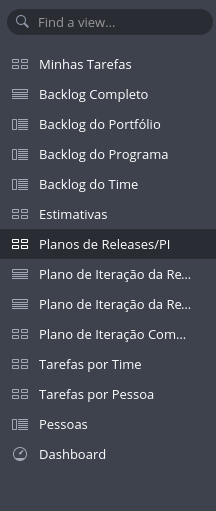
\includegraphics[width=0.2\textwidth]{figuras/quadros.png}
    \caption{Quadros Criados e Utilizados no TargetProcess}
    \label{fig:quadros}
\end{figure}

A partir do TargetProcess, também é possível visualizar o status do projeto no presente momento, com detalhes como: a porcentagem de processos já concluída, features e histórias de usuário realizadas e faltantes, bugs e os criadores/desenvolvedores. Exemplo na próxima imagem.

\begin{figure}[!htb]
    \centering
    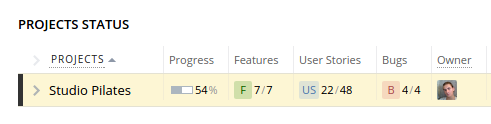
\includegraphics[width=0.7\textwidth]{figuras/status_projeto.png}
    \caption{Status do Projeto}
    \label{fig:status_projeto}
\end{figure}

Além disso, na imagem seguinte, é possível visualizar também o Gráfico Burn Down (também gerado a partir do TargetProcess) que representa diariamente o progresso do trabalho em desenvolvimento. O gráfico da equipe revela o esforço da equipe apesar de estar sempre a frente da linha recomendada, estando em evolução. Portanto, o ritmo de trabalho foi adequado para atingir a meta da Sprint 1.

\begin{figure}[!htb]
    \centering
    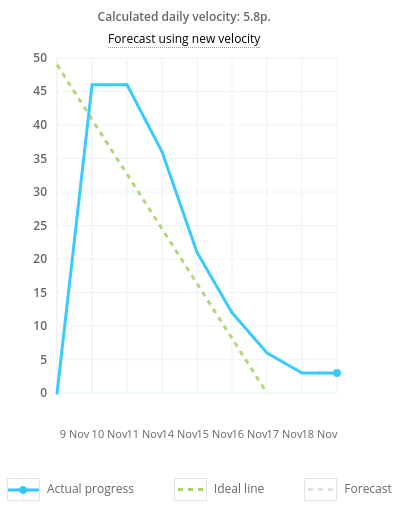
\includegraphics[width=0.5\textwidth]{figuras/burn_down.png}
    \caption{Gráfico Burn Down}
    \label{fig:burn_down}
\end{figure}
\chapter[Relatos de Experiência]{Relatos de Experiência}

\section[Execução de Trabalho]{Execução de Trabalho}

\section[Disciplina de Engenharia de Requisitos]{Disciplina de Engenharia de Requisitos}

\chapter[Conclusão]{Conclusão}

\chapter[Referências Bibliográficas]{Referências Bibliográficas}

Agile Manifesto (2001) Manifesto para Desenvolvimento Ágil de Software. Disponível em: <http://agilemanifesto.org/iso/ptbr/>. Acesso em: 02 nov. 2016.

AMBLER, S. W. Agile Requirements Best Practices. Agile Modeling. Disponível em: <http://www.agilermodeling.com/essays/agileRequirementsBestPractices.htm>. Acesso em 02 nov. 2016.

AMBLER, S. W. Introduction to User Stories. Agile Modeling. Disponível em: <http://www.agilermodeling.com/artifacts/userStory.htm>. Acesso em 02 nov. 2016.

AURUM, A., WOHLIN, C., Engineering and Managing Software Requirements, Springer-Verlag, 2005. 

BELGAMO, Anderson; Martins, Luiz. E. G; Um Estudo Comparativo sobre as Técnicas de Elicitação de Requisitos do Software, XIX CTIC (Concurso de Trabalhos de Iniciação Científica) no XX Congresso Brasileiro da Sociedade Brasileira de Computação, Curitiba, 2000.

GOTEL, O. e FINKELSTEIN, A., “An analysis of the Requirements Traceability Problem,” in Proceedings of the First International Conference on Requirements Engineering, (Colorado springs, CO), pp. 94-101, April 1994.

KIRAWOWSKI, J; Requirements Engineering and Specification in Telematics: Methods for User-Orientated Requirements Specification. Human Factors Research Group, Cork, Ireland,1997. Disponível em http://www.ejeisa.com/ nectar/respect/3.2/.

KOTONYA, G., SOMMERVILLE, I., Requirements engineering: processes and
techniques. Chichester, England: John Wiley, 1998. 

LEFFINGWELL, D. Agile Software Requirements: Lean Requirements Practices for Teams, Programs, and the Enterprise, Capítulo 12, 2010.

MENDES, L. M.; COSTA, R. H.; LOURENSO, R. O Gerenciamento de Requisitos e a sua Importância em Projetos de Desenvolvimento de Software. Instituto Federal de Educação, Ciência e Tecnologia de São Paulo, 2015.

POHL, Klaus; Rupp, Chris. “Requirements engineering fundamentals: A study guide for the certified professional for Requirements Engineering exam: Foundation level, IREB compliant”. 1.ed, 2012

Portal DevMedia. Disponível em: http://www.devmedia.com.br/engenharia-de-software-2-tecnicas-para-levantamento-de-requisitos/9151. Acesso em 25 de outubro de 2016.

ROBERTSON, S., ROBERTSON, J. Mastering the Requirements Process. 2nd Edition. Addison Wesley, 2006.

SAFe Framework. Disponível em: http://www.scaledagileframework.com/. Acesso em 25 de outubro de 2016.

SILLITTI, A.; HAZZAN, O.; BACHE, E.; ALBALADEJO, X. Agile Processes in Software Engineering and Extreme Programming: 12th International Conference, XP 2011, Madrid, Spain, May 10-13, 2011.

SOMMERVILLE, I. Engenharia de Software, 8a edição. Tradução: Selma Shin Shimizu Melnikoff, Reginaldo Arakaki, Edilson de Andrade Barbosa; São Paulo: Pearson Addison-Wesley, 2007.

WIEGERS, K.E., Software Requirements: Practical techniques for gathering and managing requirements throughout the product development cycle. 2nd Edition, Microsoft Press, Redmond, Washington, 2003. 




Referências Bibliográficas
\input{editaveis/textoepostexto}
\input{editaveis/elementosdotexto}
\input{editaveis/elementosdopostexto}
\bookmarksetup{startatroot}
\postextual
\bibliography{bibliografia}
\input{editaveis/apendices}
\begin{anexosenv}
\partanexos
\chapter{Primeiro Anexo}
A figura abaixo se refere a primeira parte do modelo de contrato usado na empresa.
\begin{figure}[h!]
    \centering
    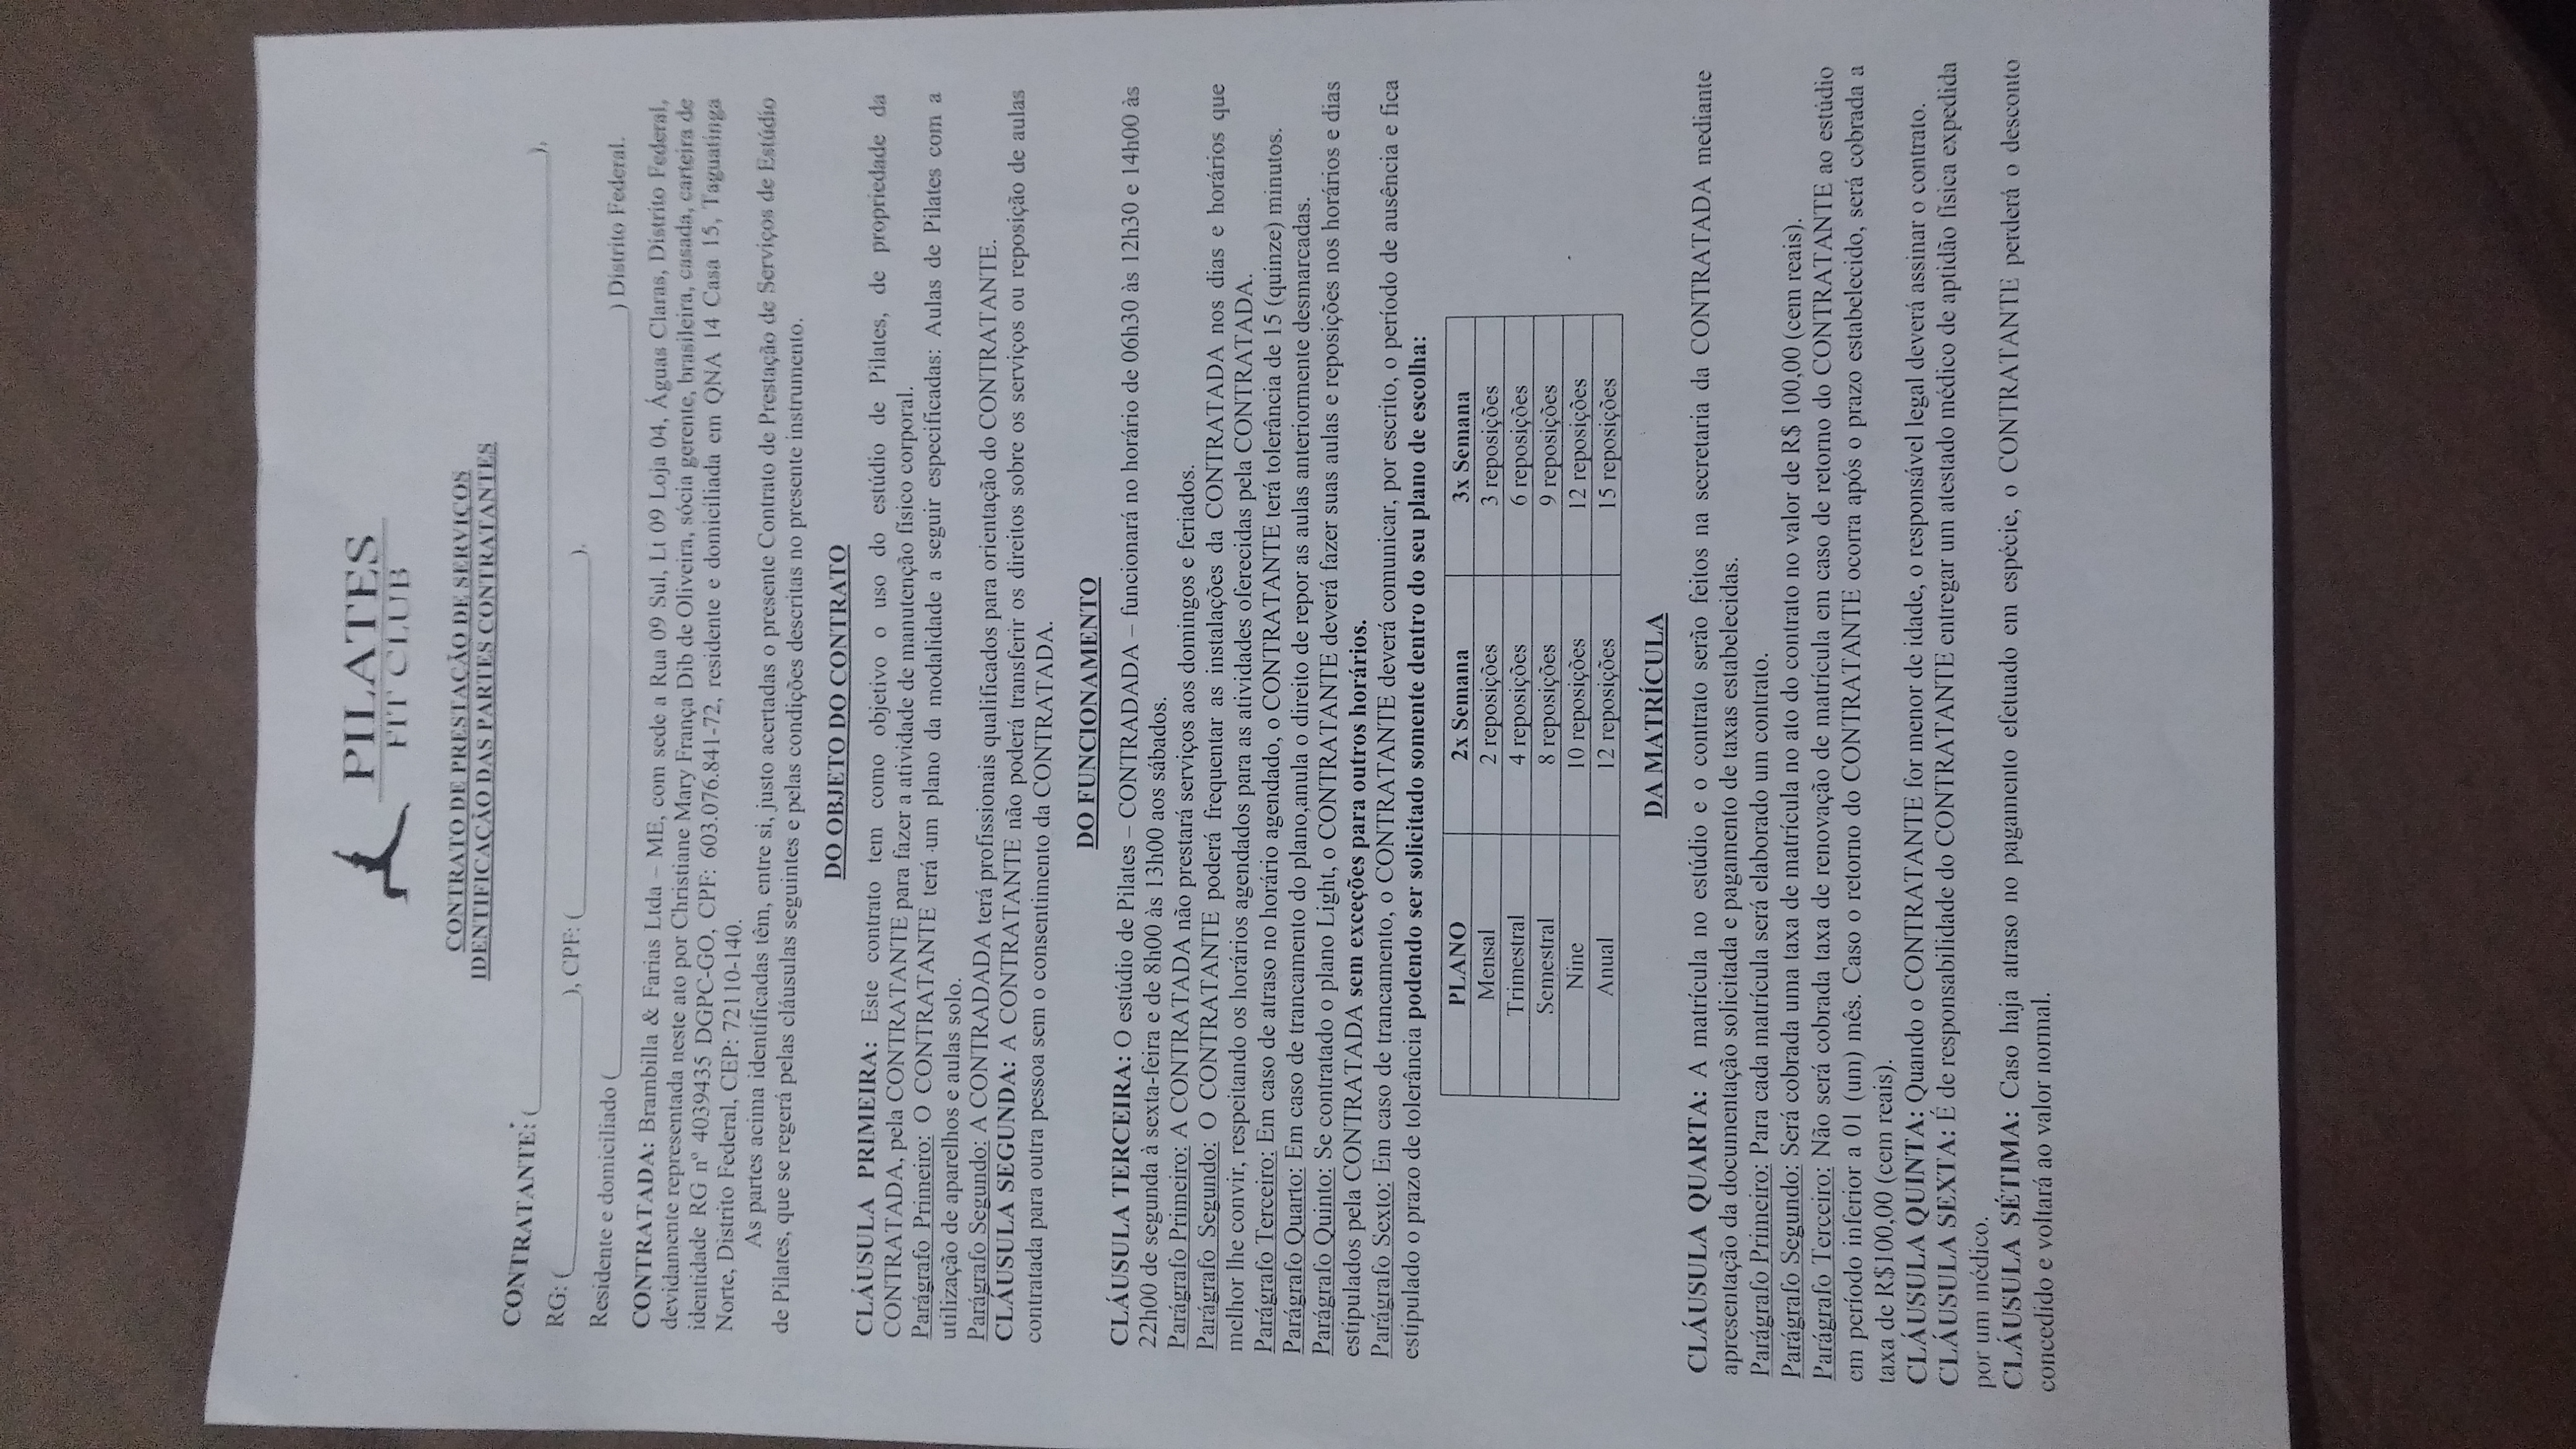
\includegraphics[width=\textwidth, angle=-90]{figuras/contrato_1.jpg}
    \caption{Plano de Contrato, página 1.}
    \label{fig:contrato_1}
\end{figure}
\chapter{Segundo Anexo}
A figura abaixo se refere a segunda parte do modelo de contrato usado na empresa.
\begin{figure}[h!]
    \centering
    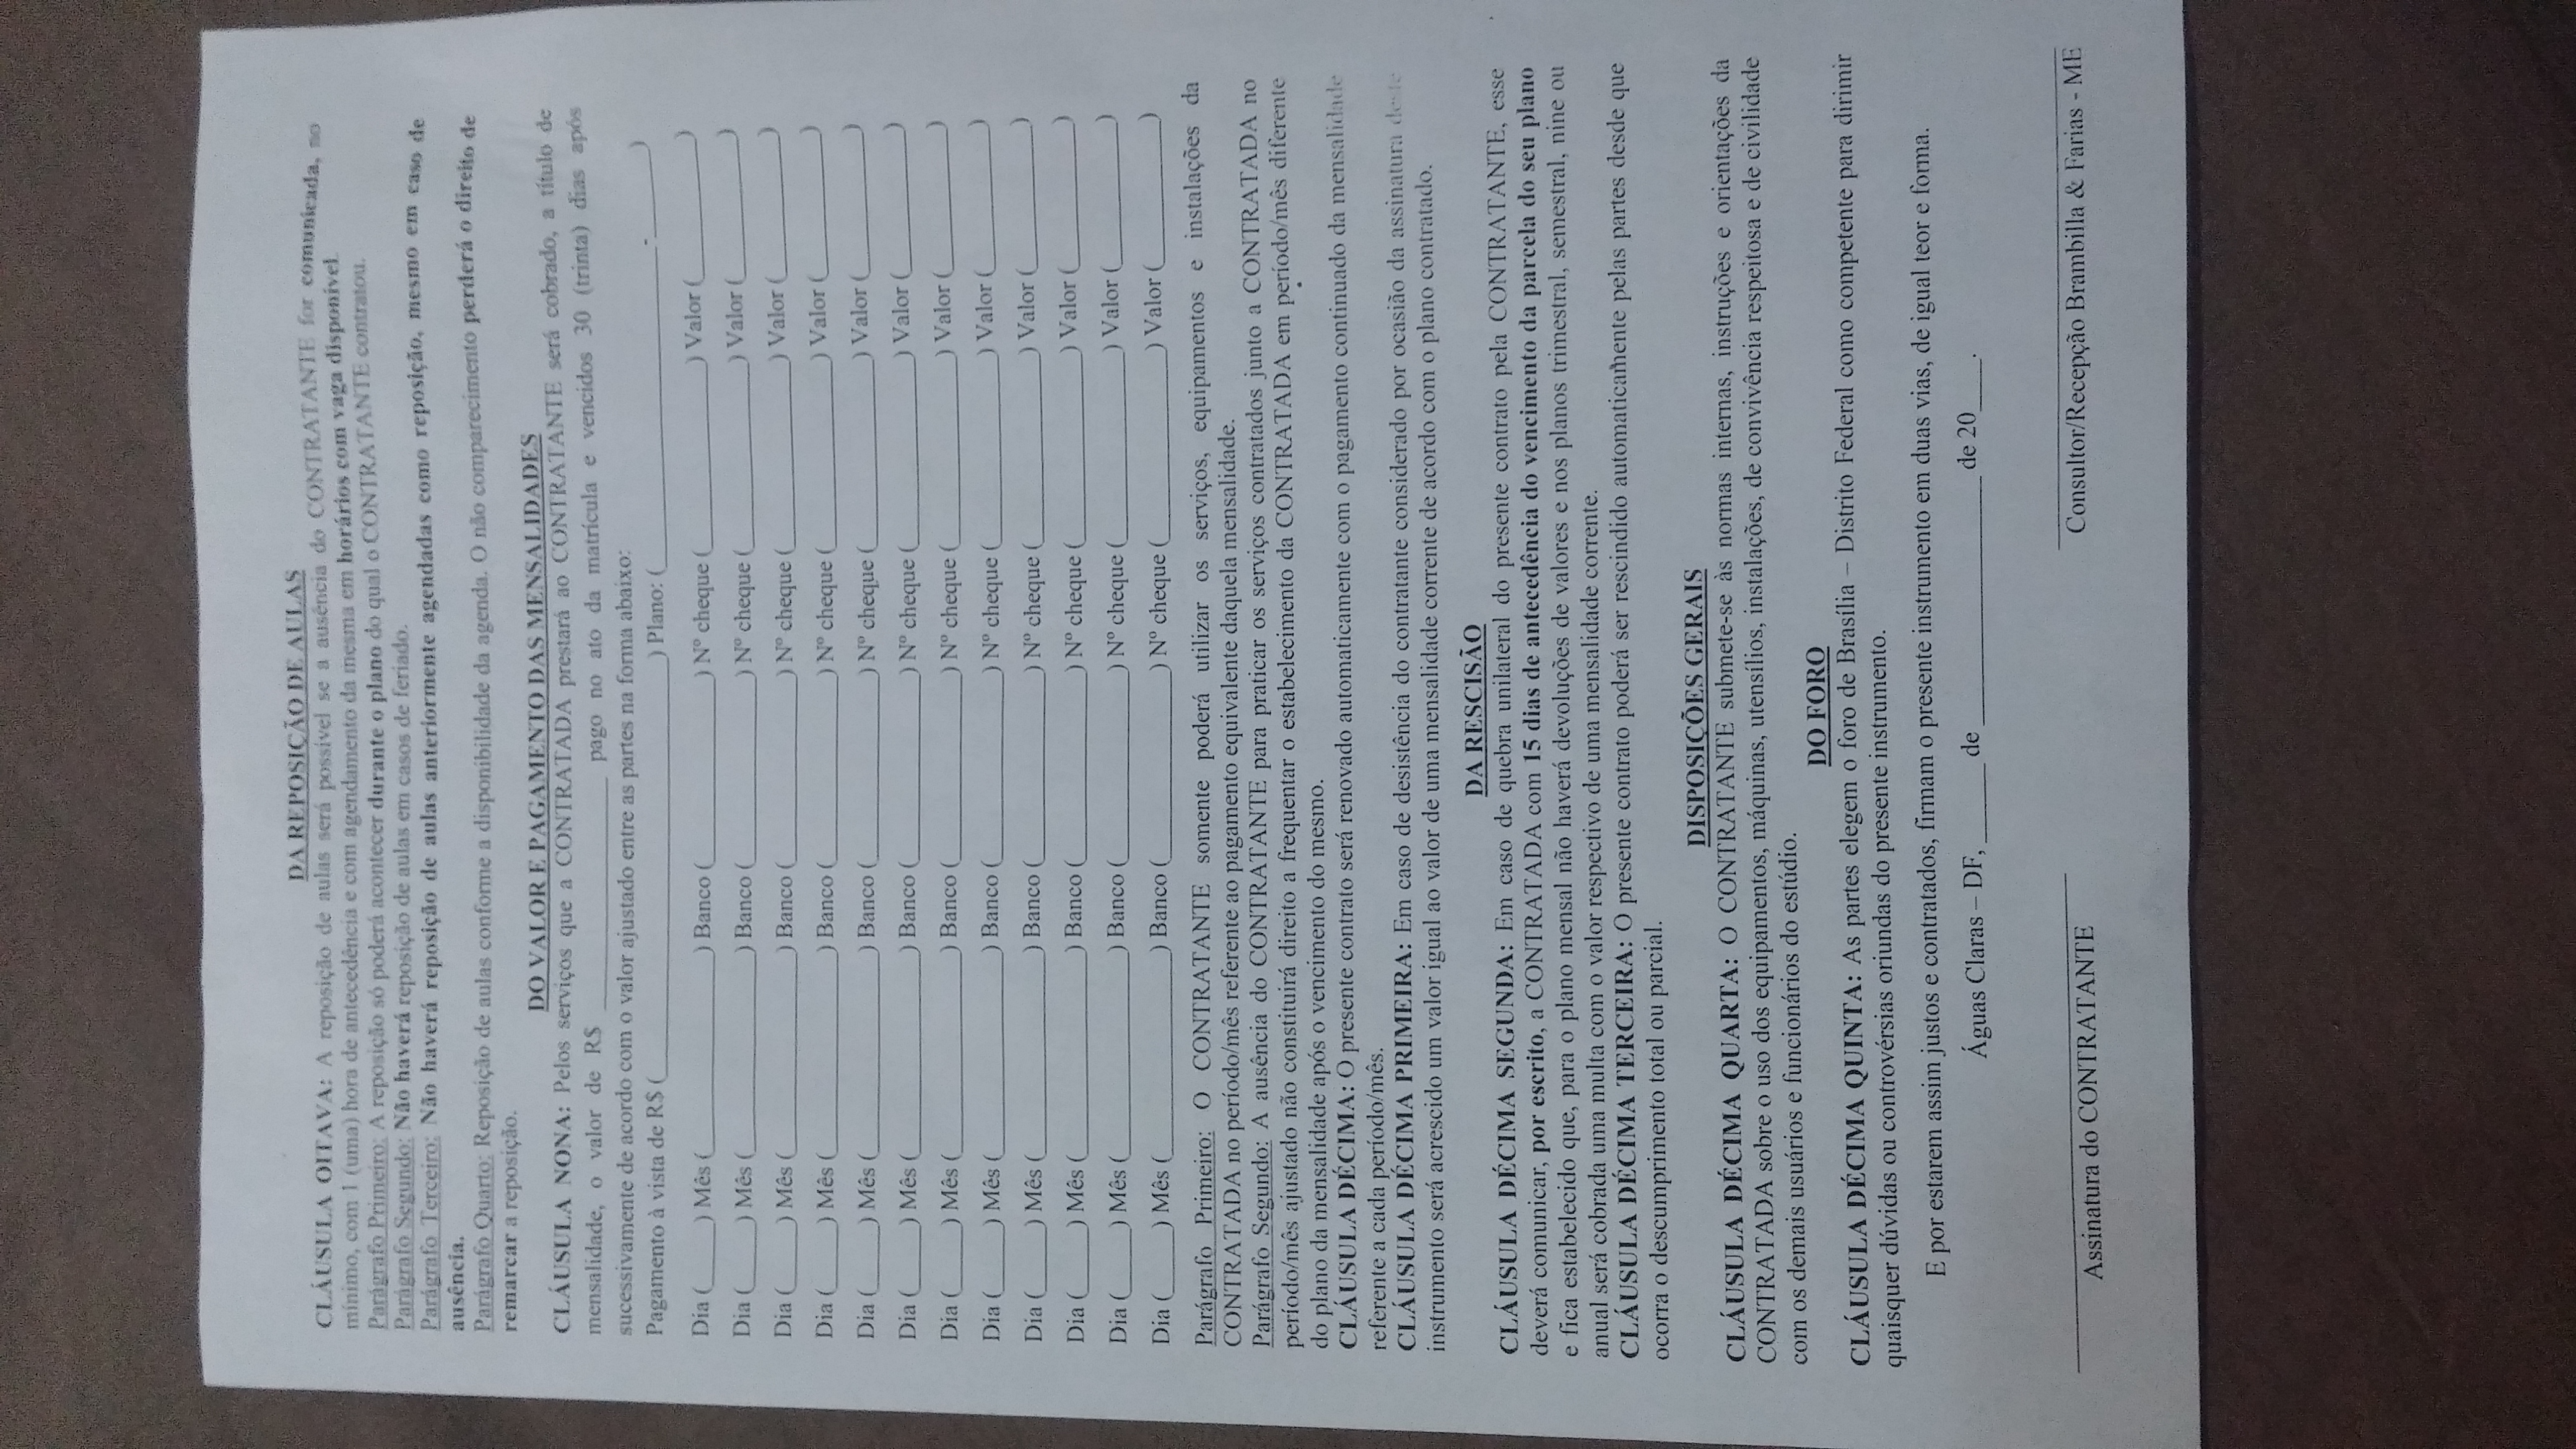
\includegraphics[width=\textwidth, angle=-90]{figuras/contrato_2.jpg}
    \caption{Plano de Contrato, página 2.}
    \label{fig:contrato_2}
\end{figure}
\chapter{Terceiro Anexo}
Esse anexo se refere a ficha de matrícula que a empresa utiliza.
\begin{figure}[h!]
    \centering
    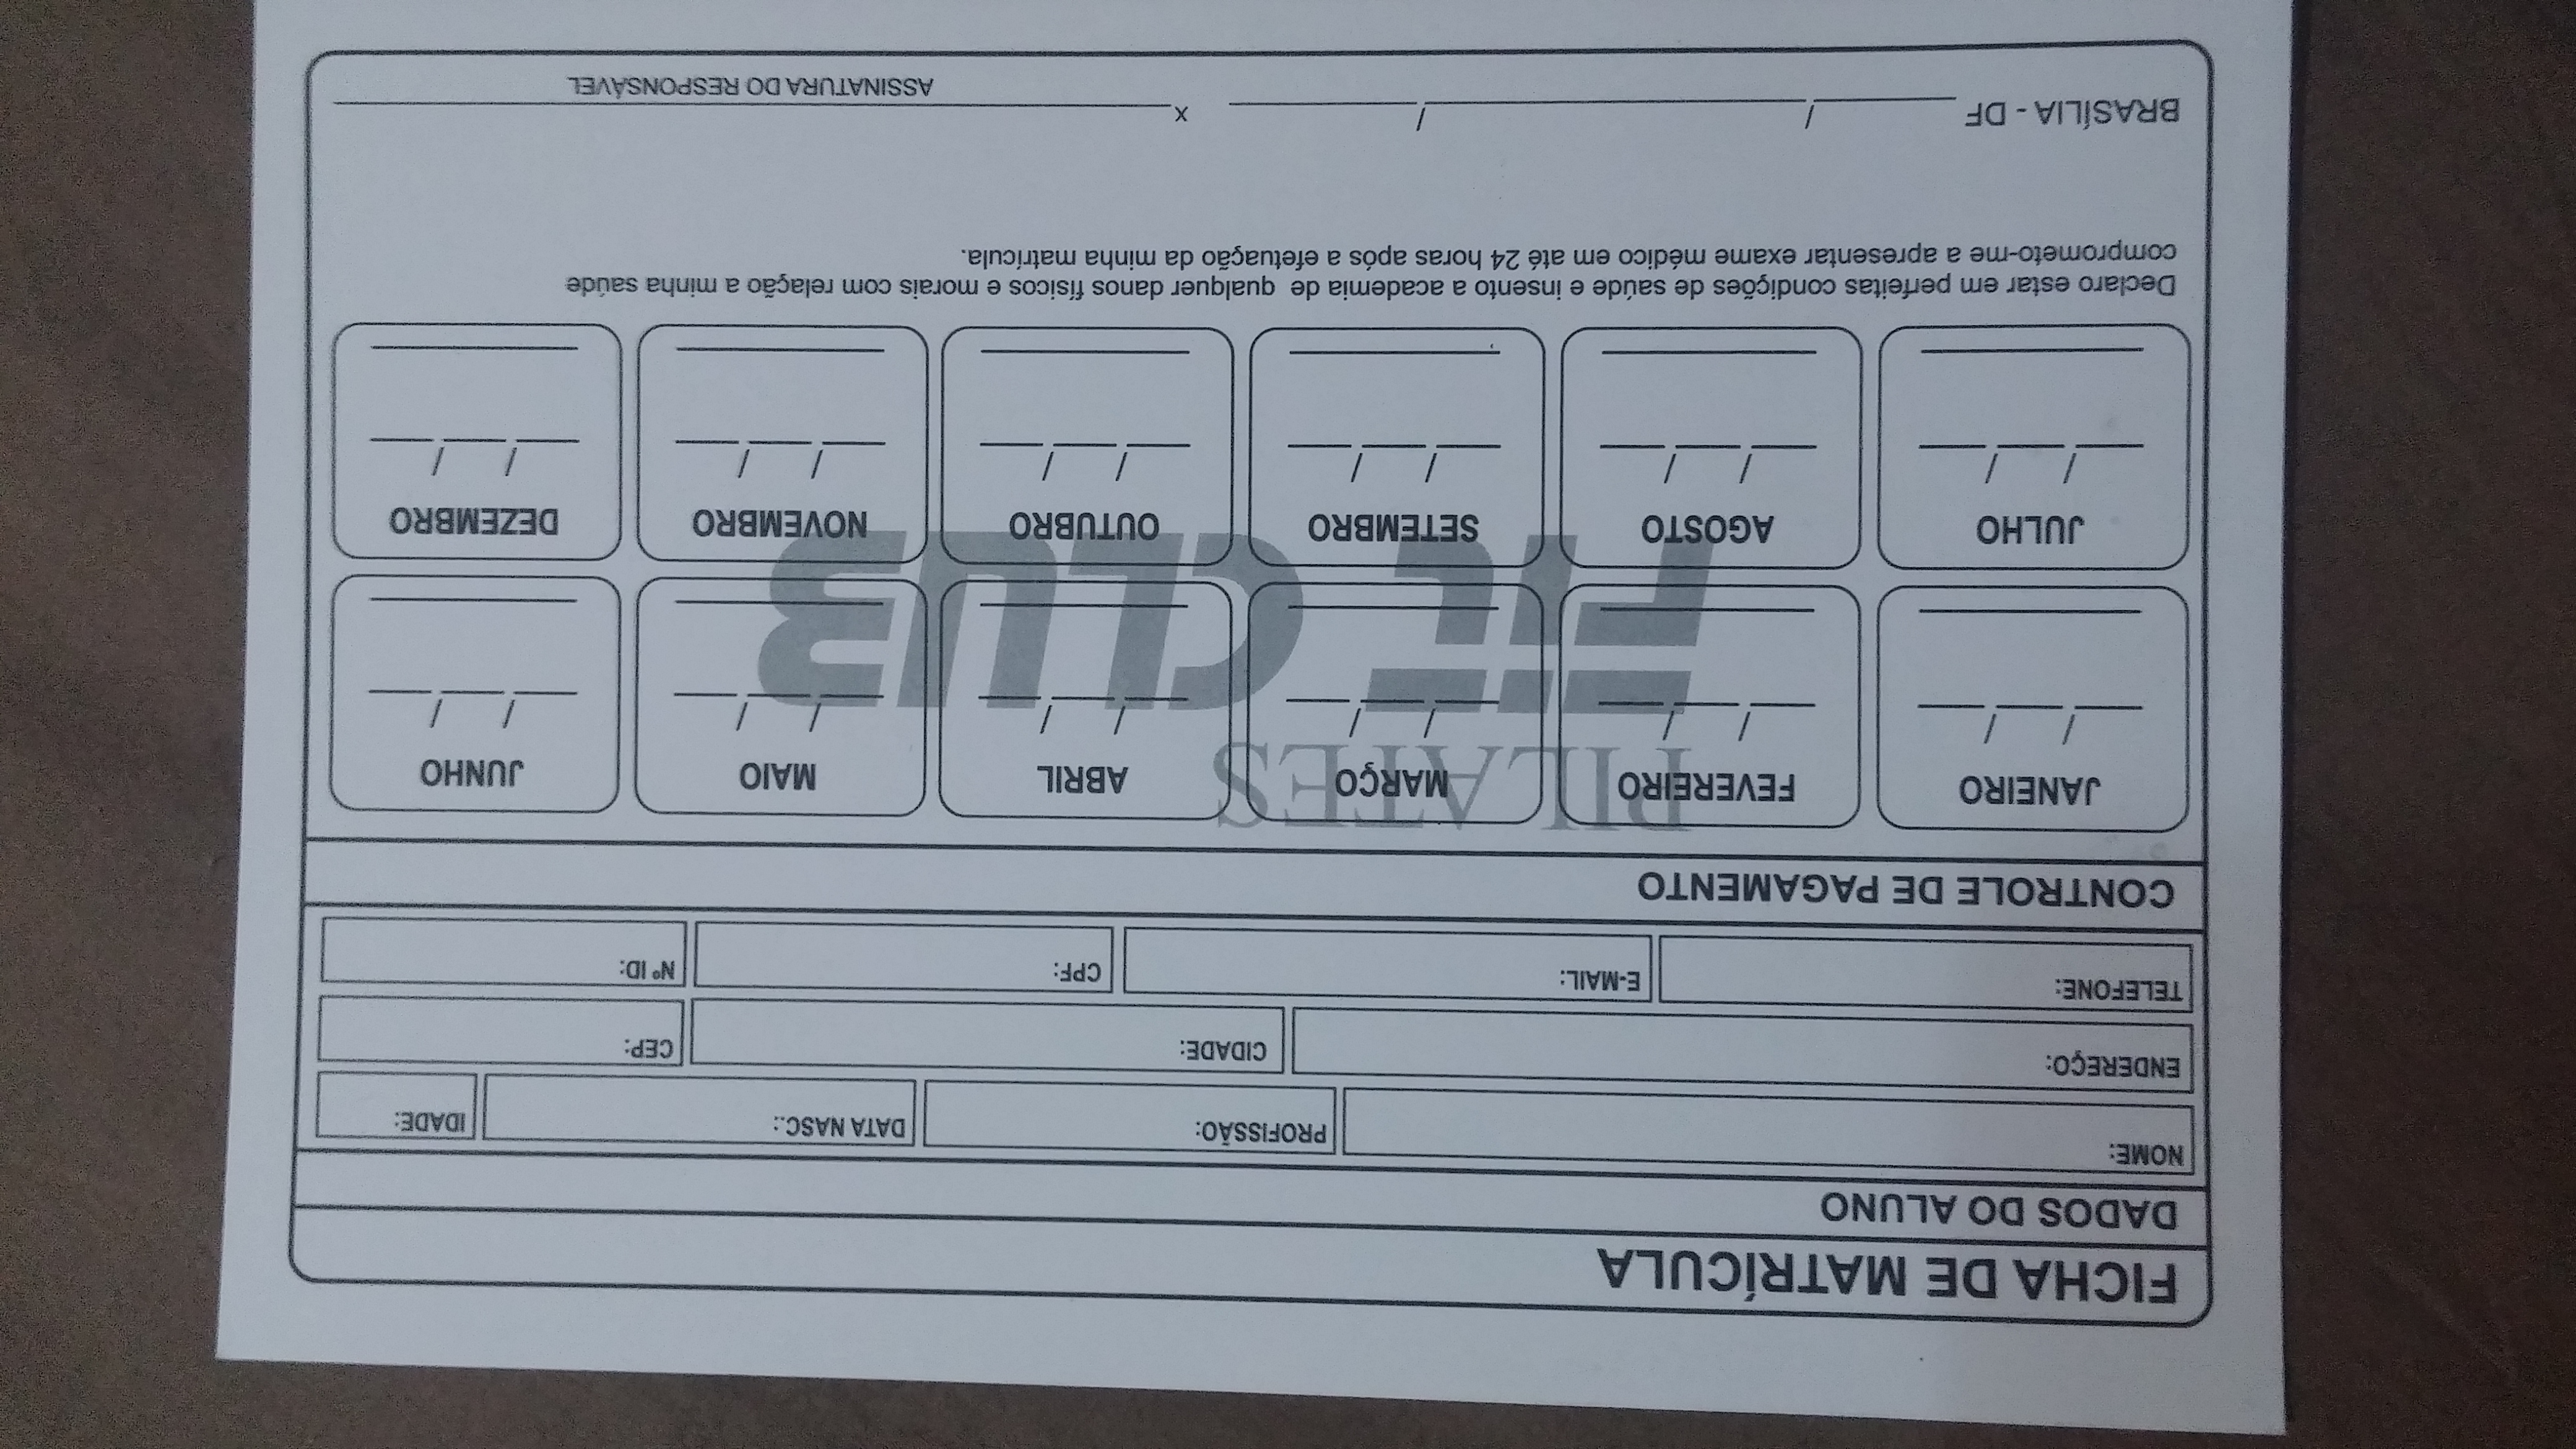
\includegraphics[width=\textwidth, angle=-90]{figuras/matricula.jpg}
    \caption{Ficha de matrícula.}
    \label{fig:matricula}
\end{figure}
\chapter{Quarto Anexo}
Esse anexo mostra como é feito o controle de vencimentos na empresa.
\begin{figure}[h!]
    \centering
    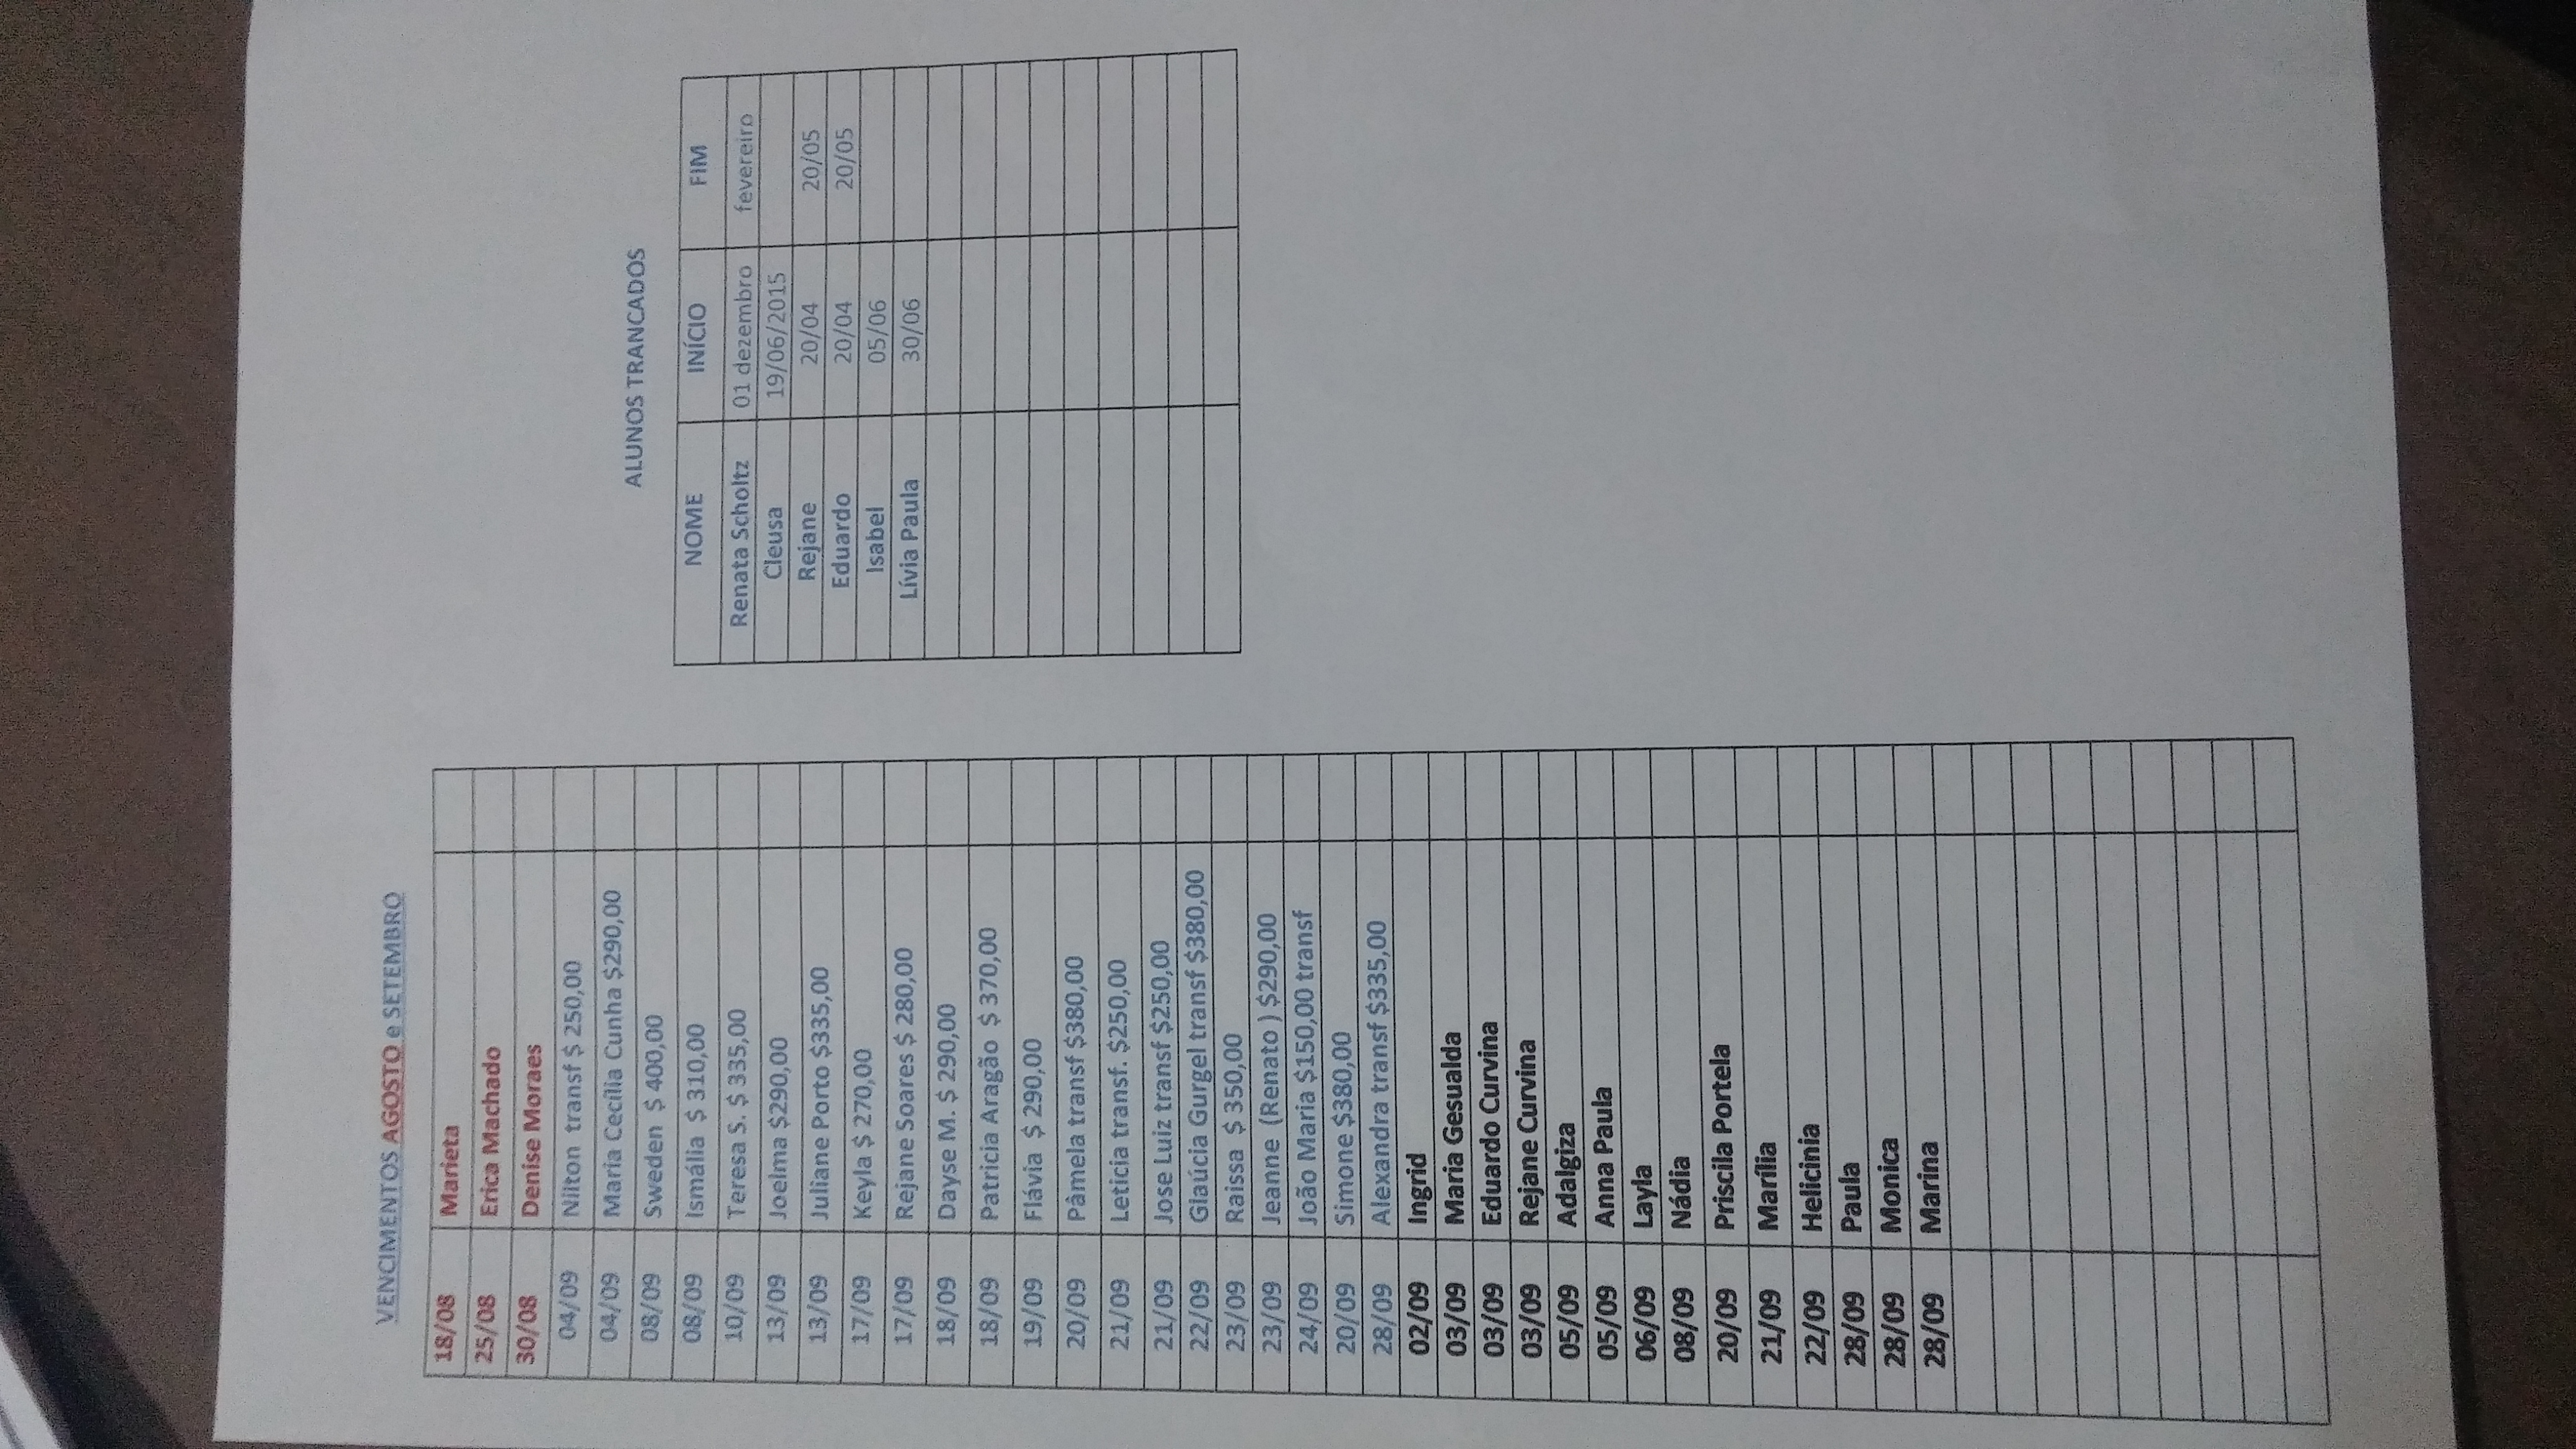
\includegraphics[width=\textwidth, angle=-90]{figuras/vencimentos.jpg}
    \caption{Tabela de vencimentos.}
    \label{fig:vencimentos}
\end{figure}
\end{anexosenv}

\printindex

\end{document}
